\documentclass[12pt, a4wide]{scrreprt}

\usepackage{scrhack}
\usepackage{scrpage2}
\usepackage{graphicx}
\usepackage[utf8]{inputenc}
\usepackage{ngerman}
\usepackage{multicol}
\usepackage[printonlyused,withpage]{acronym}

\usepackage{titlesec}

%numbers braucht man wohl für IEEEtranN...
\usepackage[numbers]{natbib}

\begin{document}
\setkomafont{disposition}{\normalcolor\bfseries}
%-------Titelseite-------%
\noindent
Konstantin Obermann \hfill Mat.nr: 947545\\
Universität Osnabrück \hfill 23.10.2015\\
Wintersemester 15/16\\
\thispagestyle{empty}
\begin{center}

\includegraphics[scale=.9]{uos_proper.png}
\section*{}
{\LARGE Ausarbeitung zum Thema}\\
\section*{}
{\Huge {\bf Lokalisierung in drahtlosen Sensornetzwerken}}\\
\section*{}
{\Large Im Rahmen des Seminars ''Verteilte Systeme''}\\
\section*{}
{\Large Betreuer:}\\
{\Large Prof.Dr.rer.nat Nils Aschenbruck}\\
{\Large Dipl.-Inform. Matthias Schwamborn}\\
\end{center}


\newpage
\pagestyle{empty}
\section*{Abkürzungsverzeichnis}
 \begin{acronym}
\acro{WSN}{Wireless Sensor Network}
\acro{AOA}{Angle of Arrival}
\acro{RSS}{Received Signal Strength}
\acro{TOA}{Time of Arrival}
\acro{TDOA}{Time Difference of Arrival}
\acro{COTS}{Commercial Off-The-Shelf}
\end{acronym}

\newpage
\tableofcontents
\pagenumbering{roman}

%-------Einleitung-------%
\chapter{Einleitung und Motivation}
\pagenumbering{arabic}
Der technologische und wirtschaftliche Fortschritt erfordert eine zuverlässige, konsistente und in vielen Fällen drahtlose Kommunikation. Beispiele für drahtlose Netzwerke sind Mobilfunknetzstandards GSM, UMTS und LTE oder das drahtlose Netzwerkprotokoll WLAN.\\
\indent
Diese Ausarbeitung beschäftigt sich hauptsächlich mit den \ac{WSN}.

\indent
Die Lokalisierung der einzelnen Sensorknoten innerhalb WSNs erfolgt auf Basis von \ac{AOA}, \ac{RSS} oder distanzbasierten Ansätzen zur Positionsbestimmung. Eine schnelle Lokalisierung der einzelnen Sensoren erfolgt dann, wenn diese vorher optimal platziert werden, um die Anzahl an Knoten im WSN zu minimieren und den Overhead in den Lokalisierungsalgorithmen zu vermeiden\cite{area_based}.\\
\indent
Faktoren, wie Schnelligkeit und Präzision der Lokalisierung sowie der Grad der Autonomie des WSN, beeinflussen dessen Zuverlässigkeit und Potential. Dieses Potential ist entscheidend für die Auswahl an Einsatzmöglichkeiten eines WSN. Das Erdbeben-Frühwarnsystem (EEW) ist eines der Einsatzmöglichkeiten. Hier ist eine reibungslose und schnelle Kommunikation zwischen den Knoten besonders wichtig, denn ein Fehlalarm ist kostspielig. Allerdings ein im Ernstfall verspäteter Alarm kann Menschenleben kosten. Weitere Beispiele für die Verwendung von Sensornetzen sind Erkennung von Waldbränden, Überwachung von Deichen, Überwachung von Gebäudestatik, um Erdbebenschäden zu erkennen\cite{building_monitoring} oder das ''Precision Farming''. Bei dem letzten Beispiel werden Sensorknoten auf einem landwirtschaftlich genutzten Feld verteilt, damit sie die Luftfeuchtigkeit, Temperatur und Grundwasserspiegel messen können. Diese Messungen sollen die Produktivität der Ernte steigern.\\
\indent
Zusätzlich zu den auftretenden Messfehlern treten natürliche Störfaktoren auf, die ein Problem darstellen und eine wichtige Rolle bei der Entwicklung und Optimierung dieser Lokalisierungstechniken spielen.

\chapter{Wireless Sensor Networks: Die Grundlagen}

Die WSNs bestehen aus kleinen, vergleichsmäßig leistungsschwachen Sensoren, welche als Knoten (engl. nodes) in dem WSN dienen. Ein Beispiel dafür ist das \textit{WiSe Mote} mit einer Größe von 56x58mm, ausgestattet mit einem \textit{ZigBee 2420} drahtlosen Kommunikationsmoduls und in den Mikrocontroller eingebauten 4kB RAM\cite{WiSe}.\\
\indent
Die Lebensdauer der Knoten reicht i.d.R. von 100-200 Stunden\cite{lifetime_study} bis zu 40 Jahren.\\
\indent
Einige Anwendungsbereiche erfordern einen zentralen Rechner. In diesem Fall sollte also ein- oder mehrere Knoten als Gateway konfiguriert werden, um klar definierte Schnittstelle(n) zur Zentrale zu bilden.\\
\indent
Zwar kann die Position der Knoten mit dem GPS ermittelt werden, allerdings erfordert die Vielseitigkeit der Einsatzmöglichkeiten der WSN eine Unabhängigkeit von der GPS-Positionierung. Das liegt daran, dass das GPS trotz der genauen Ortung ein zu schwaches Funksignal nutzt, welches eine zuverlässige  Ortung innerhalb von Gebäuden oder unter der Erde nicht möglich macht. Deswegen muss ein WSN in der Lage sein, eigenständig ein Netz zu initialisieren, alle Nichtanker-Knoten zu orten und ggf. deren Standortinformationen an einen zentralen Rechner weiterzugeben.

%\chapter{Die richtige Ankerplazierung}
%Die richtige Plazierung der Anker spielt eine große Rolle bei den meisten %Lokalisierungsmethoden.

\chapter{Ansätze zur Positionsbestimmung}
Bei den Knoten im WSN unterscheidet man zwischen \textit{Ankerknoten} bzw. \textit{Anker}, deren absolute Position initial bekannt ist und den \textit{Sensorknoten}, deren Position mithilfe der Anker bestimmt werden soll. 
Die weitere Ausstattung und somit die Kosten und Komplexität der Sensoren hängt von der Lokalisierungsmethode ab.\\
\indent
Die Hardware der Sensorknoten ist in der Regel den Anwendungsbereichen angepasst. Da die Sensorausstattung ebenso von der Lokalisierungsmethode abhängt, hat die Wahl des passenden Ansatzes einen großen Einfluss auf die Kosten und den Energieverbrauch der Sensoren. Die Ansätze lassen sich in zwei grobe Kategorien einteilen\cite{area_based}.\\
\indent
Die erste Kategorie umfasst die \textit{range-based} Methoden, welche mit Abstands- oder Winkelmessung arbeiten. Diese nutzen die im weiteren Verlauf beschriebenen Ansätze wie AOA, TOA, TDoA, RSS und erreichen, auf Kosten von Komplexität, eine höhere Genauigkeit als die zweite Kategorie.\\
\indent
In die zweite Kategorie fallen die \textit{range-free} Methoden, also Lokalisierungstechniken, die auf einen direkten Bezug zwischen einem Anker und einem Sensorknoten verzichten. Hierbei gibt es unterschiedliche Methoden und eine davon ist \textit{area-based}\cite{area_based}. Das Prinzip hierbei ist, dass die Anker mithilfe von unterschiedlich empfangenen Signalstärken untereinander eine Fläche generieren, in welcher die Position des Senders geschätzt werden soll.\\
\indent
Die range-based Methoden eignen sich für WSNs, bei denen eine möglichst exakte Positionsbestimmung wichtig ist. Die range-free Lokalisierung ist eine Alternative, wenn die Ausstattung der Knoten im WSN möglichst kosteneffizient sein soll und die Kenntnis über die exakte Position der Sender nicht zwingend erforderlich ist.\\ 
\indent
Im Folgenden werden die grundlegenden Ansätze zur Positionsbestimmung vorgestellt.

\section{Range-free Methoden}
\section{Range-based Methoden}
  \subsection{Angle Of Arrival Ansätze}
Das Prinzip der {\bf A}ngle {\bf O}f {\bf A}rrival (AOA) Lokalisierung arbeitet mit dem Eintrittswinkel des empfangenen Signals. Dazu sollte der Empfänger einen ungehinderten Sichtkontakt zum Sender haben. Diese Lokalisierungsart kann in zwei Vorgehensweisen aufgeteilt werden, die in den Folgenden zwei Kapiteln beschrieben werden.  
  \subsection*{Das Beamforming Prinzip}
Beim Beamforming wird mithilfe einer Richtanenne ein ankommendes Signal normiert, indem der Empfangskegel der Richtanenne mechanisch oder elektronisch gedreht wird, bis das empfangene Signal die höchste Sendeleistung erreicht. Somit kann die Richtung des Senders bestimmt werden. Eine variierende Signalstärke ist ein Störfaktor bei dieser Methodik. Ein Ansatz, welcher in \cite{q1} besprochen wird, befasst sich mit mehreren rotierbaren Richtantennen, deren gesammelten Informationen durch eine zentrale Einheit überlappt berechnet werden und somit eine höhere Genauigkeit erreicht werden. Laut \cite{q1} können mit 4 Richtantennen eine Richtungsgenauigkeit von $10^\circ -15^\circ$, mit 6 Antennen $5^\circ$ und mit bereits 8 Antennen eine Genauigkeit von $2^\circ$ erreicht werden.
    \subsection{Phase Interferometry}
Mithilfe des \textit{phase interferometry}\cite{q1} Verfahrens lässt sich die Richtung eines eingehendes Signals durch eine Antennenfront bestimmen. In {\bf Abb.3.1} ist der Aufbau skizziert. Hierbei sind $x1...xn$ die Antennen, welche mit dem gleichen Abstand $d$, welcher vorher bekannt ist, zueinander aufgebaut sind. Diese Antennen empfangen das Signal des Senders zu unterschiedlichen Zeitpunkten. Während die letzte Welle in diesem Beispiel gerade noch $x1$ verlässt, so tritt sie gleichzeitig bei $x2$ ein. Das ist der zeitliche Unterschied der empfangenen Phase, also die \textit{Phasenverschiebung}. Mithilfe dieses Phasenunterschiedes lässt sich mathematisch die Richtung des Senders bestimmen.\\

\begin{figure}[!htb]
\centering
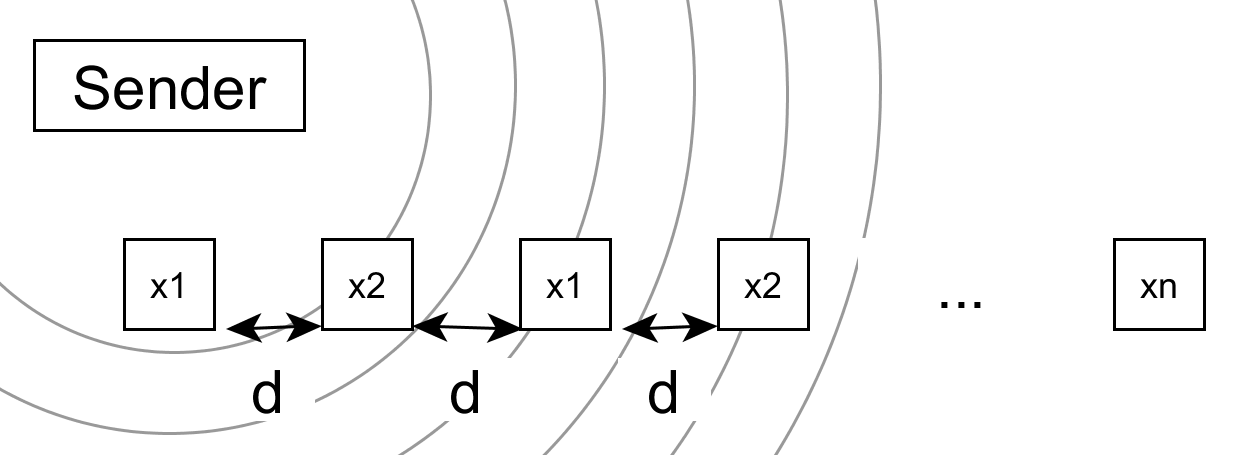
\includegraphics[scale=.3]{phase_int2.png}
\caption{Ankommende Wellenfronten an den Antennen}
\end{figure}

  \section{Distanzbasierte Ansätze}
Bei den distanzbasierten Ansätzen werden Informationen genutzt, mit deren Hilfe sich der Abstand zur Signalquelle berechnen lässt. Die Übertragungszeit eines Signals vom Sender zum Empfänger ist eine Information, welche genutzt werden kann, sowie die Übertragungs- und Rückkehrzeit (auch \textit{ping} genannt).
    \subsection{Lighthouse Approach}
Das Verfahren, das dem \textit{Lighthouse approach} zugrunde liegt, basiert auf dem Prinzip eines Leuchtturms. Das Licht eines Lechtturms strahlt gerichtet und dreht sich um seine Achse, damit es von allen Seiten gesehen werden kann.\\
\indent
Für dieses Ortungsverfahren wird ein Sender benötigt, welcher als Leuchtturm fungiert. Die Empfänger des Signals müssen mit hoher Präzision arbeiten, also sollte das Licht des Senders ebenfalls möglichst ohne Abweichungen verlaufen. In {\bf Abb.3.2} ist der grobe Aufbau des \textit{Lighthouse approach} skizziert. Man kann erkennen, dass der Sender {\bf S} einen Strahl mit konstanter Breite {\bf b} ausstrahlt und sich um seine Achse dreht.\\

\begin{figure}[!htb]
\centering
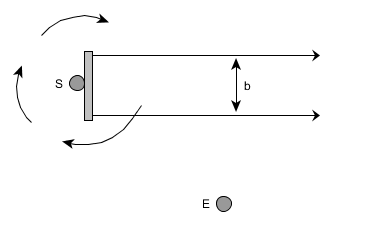
\includegraphics[scale=.78]{lighthouse.png}
\caption{Lighthouse Approach}
\end{figure}

Die Drehgeschwindigkeit des Senders ist vorher bekannt. Der Empfänger {\bf E} ist in Sichtweite aufgestellt und misst den Zeitunterschied zwischen dem Eintritt des Lichtsignals und dessen Austritt. Mithilfe der Drehgeschwindigkeit und der Zeit, die der Empfänger im Licht misst, kann die Entfernung berechnet werden.\\
\indent
Eine Möglichkeit, das Licht zu emittieren ist es, eine ausreichend breite parallele Lichtquelle zu nutzen. Parallel bedeutet, dass die Breite des Lichts unabhängig von der zurückgelegten Strecke möglichst konstant bleibt. Wie in \cite{lighthouse} beschrieben, ist dieses Vorgehen allerdings aufgrund von beschränkten Mitteln und Kapäzitäten der WSN Sensoren recht fehleranfällig und so wird z.B. ein 10cm breites Licht auf eine Entfernung von 5m eine Breite von 18.7cm erreichen.\\
\indent
Als Alternative ist es möglich, zwei Laser am Sender so anzubringen, dass sie einen in eine Richtung gerichteten, parallelen optischen Strahl mithilfe von vertikal und horizontal verstellbaren Spiegeln simulieren. Mit der COTS Hardware lässt sich eine Drehfrequenz von bis zu 300Hz\cite{lighthouse} erreichen. 
\newpage
    \subsection{One-Way Propagation/Time of Arrival}
\textit{One-Way Propagation} steht für die Übertragung eines Signals in eine Richtung. Im Gegensatz zum \textit{Round-Trip} wird das Messsignal nicht zurück gesendet. Um die Zeit zwischen dem Senden und Empfangen zu messen, muss der Empfänger die Uhrzeit des Sendens wissen. Dafür müssen die Uhren vom Sender und Empfänger möglichst synchron laufen, dies erfordert aber eine weitere, komplexe Kommunikation zwischen den Geräten. Unter dem Kosten- und Ressourcenaspekt ist dies schwierig umzusetzen.
	\subsection{Round-Trip Propagation/ping}
Die erweiterte Alternative zu One-Way Propagation ist das \textit{ping} Prinzip. Hierbei wird das Signal nicht vom Empfänger gemessen. Stattdessen sendet der Empfänger das Signal wieder zurück und der ursprüngliche Sender vergleicht die Sende- und Rückkehrzeit des Signalpakets. Anhand dieser Zeitdifferenz lässt sich dann die Distanz berechnen. Hierbei wird keine Synchronisierung der Sender- und Empfängeruhren benötigt. Der Empfänger braucht allerdings eine bestimmte Zeit, um das Signal zu empfangen, verarbeiten und wieder zurückzuschicken. Diese Zeit kann der Empfänger selbst ausrechnen und zurückschicken, damit die Berechnungen um diesen Wert korrigiert werden können.\\
    \subsection{Time Difference Of Arrival}
    \subsection{RSS-basierte Lokalisierung}    
  \section{Flächenbasierte Lokalisierung}
Die flächenbasierte Lokalisierung ist eine Spezialform der \textit{range-free} Lokalisierungsansätze.
\chapter{Einsatzmöglichkeiten}
  \section{Kommerzieller Einsatz}
  \section{Industrieller Einsatz}

\chapter{Aktuelle Probleme und Fragestellungen}
  \section{Multipath propagation}
\textit{Multipath propagation}(Mehrwegempfang) ist eines der Störfaktoren in der drahtlosen Übertragung. Dieser Faktor beeinflusst alle Messmethoden, die sich auf eine konstante Signalstärke eines oder mehrerer Empfänger verlassen müssen. Mehrwegempfang tritt auf, wenn Signal von Oberflächen reflektiert wird und somit ein gespiegeltes, schwächeres Signal entsteht. Dieses Phantomsignal kann Messergebnisse beeinflussen, weil es als eine zusätzliche Quelle wahrgenommen werden kann.
  \section{Shadowing}

\chapter{Zusammenfassung}

\newpage
\bibliographystyle{IEEEtranN}
\pagestyle{empty}
\bibliography{sources}
\nocite{*}
\end{document}